\subsection{Элементы статистической физики}
\subsubsection{Принцип детального равновесия и его применение (вывод закона Кирхгофа, связь $r_{T, \omega}^*$ vs $u_{T, \omega}$, формула Эйнштейна для коэффициентов A и B)}
\paragraph{Принцип детального равновесия.}\label{sec:teplo} В нагретых телах часть внутренней
энергии вещества может превращаться в энергию излучения. Эксперименты
показывают, что тепловое излучение имеет непрерывный спектр. Распределение
энергии излучения по спектру зависит от температуры (позже выясняется, что
максимум смещается к низким частотам с увеличением температуры, хотя общая
энергия возрастает). 

Если несколько тел окружить полостью с идеально отражающими непроницаемыми
стенками, то со временем установится \emph{тепловое равновесие}, причём оно
будет устойчивым. Зеркальные стенки можно заменить стенками из одинакового
материала с поддерживаемой температурой. В других видах излучения равновесия
быть не может.

Равновесное тепловое излучение однородно, то есть его плотность
энергии одинакова во всех точках внутри полости, где оно 
заключено. Такое излучение изотропно, однородно и неполяризованно --- оно 
содержит все возможные направления распространения и 
направления колебаний векторов $ \mathbf E $ и $ \mathbf H $.

В опыте с равновесным излучением, конечно, каждое тело будет излучать в единицу
времени столько же энергии частоты $ \omega_0 $, сколько поглощать. Это и есть
\emph{принцип детального равновесия}. Тогда отношение испускательной способности
к поглощательной одинаково для всех тел в природе и является функцией частоты и
температуры. 
\[
  \left( \frac{r_{\omega, T}}{a_{\omega, T}} \right)_1 = \left( \frac{r_{\omega,
  T}}{a_{\omega, T}} \right)_2 = \ldots = \frac{r^\ast_{\omega, T}}{1} =:
  f(\omega, T).
\]
Аналогичная цепочка равенств, конечно, справедлива и для длин волн. Это и есть
\emph{закон Кирхгофа}. Он может быть получен и другим опытом, где на АЧТ
маленький кусок поверхности $ d\sigma $ заменяется обычным непрозрачным телом. Этот кусок
поглащает $ a_{\omega, T} $-ую часть, а отражает $ 1 - a_{\omega, T} $. Падает на него по-прежнему $
r^\ast_{\omega, T}d\sigma $ энергии. Поглащает он $ a_{\omega, T}
r^\ast_{\omega, T} d\sigma $, а испускает $ r_{\omega, T} d\sigma $. Снова
приходим к закону Кирхгофа. Заметим, что этот подменённый кусок $ d\sigma $ для
внутреннего наблюдателя ничем не будет отражаться от остальных, поскольку
недоиспущенную энергию он будет отражать: 
\[
  d\sigma [r_{\omega, T} + (1- a_{\omega, T}) r^\ast_{\omega, T}] =
  r^\ast_{\omega, T} d\sigma.
\]

Рассмотрим куб с ребром $ l $ и зеркальными стенками. Поместим внутрь малое по
размеру АЧТ с температурой $ T $. Разложим объёмную плотность энергии  
\[
    u(T) := \frac{dW}{dV}
\]
по частотам: 
\[
  u_{\omega, T} := \frac{dW_{\omega, \omega + d\omega}}{dVd\omega}.
\]
Рассмотрим излучение вблизи элементарной площадки $ \Delta S $ этого АЧТ.

\begin{figure}[h!]
  \centering
  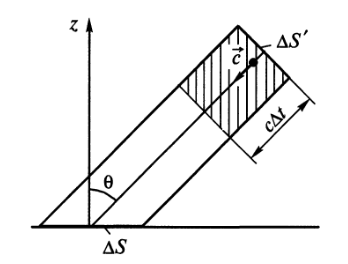
\includegraphics[width=0.4\textwidth]{img/oral-03/acht.png}
  \label{fig:acht}
\end{figure}

Плотность вблизи этой площадки равномерно распределена по всевозможным
направлениям телесного угла $ 4\pi $. Поэтому плотность энергии излучения,
приходящегося на телесный угол $ d\Omega = \sin \theta d\theta d\varphi $, то
есть падающего на площадку под углом $ \theta $ к её нормали (?), можно записать в
виде
\[
    d\tilde u = u(T) \frac{d\Omega}{4\pi}.
\]
Тогда за время $ \Delta t $ на эту площадку попадёт вся энергия излучения,
заключенная в заштрихованном объёме, то есть 
\[
    dw = d\tilde u c \Delta t \Delta S' = d\tilde u c\Delta t \Delta S \cos
    \theta = \frac{c}{4\pi} u(T)\cos \theta \sin\theta d\theta d\varphi\Delta S
    \Delta t.
\]
Найдём полный поток энергии $ \Phi $ излучения, падающего на единицу поверхности
в единицу времени: 
\[
    \Phi = \frac{c}{4\pi}u(T) \int\limits_{0}^{2\pi}d\varphi
    \int\limits_{0}^{\pi/2}\cos\theta\cdot \sin\theta\,d\theta =
    \frac{c}{4}u(T).
\]
В условиях равновесия, конечно, $ \Phi = R^\ast $. Причём данная формула
справедлива и для спектральных характеристик: 
\[
  r^\ast_{\omega, T} = \frac{c}{4}u_{\omega, T}.
\]


\paragraph{Формула Эйнштейна для коэффициентов A и B.} см. письменный вопрос \ref{einstein-a-b}

\subsubsection{Плотность квантовых состояний и плотность мод колебаний электромагнитного поля в полости}
\textbf{Плотность квантовых состояний}.
Найдём число квантовых состояний, по которым могут распределяться частицы, при
условии, что энергия этих состояний не превышает некоторого значения $ E $.
Пусть сначала частица находится в трёхмерной потенциальной яме с непроницаемыми
стенками. Энергия в такой яме равна 
\[
  E = \frac{\pi^2\hbar^2}{2m_0} \left[ \left( \frac{n_1}{a_1} \right)^2 + \left(
  \frac{n_2}{a_2}\right)^2 + \left( \frac{n_3}{a_3} \right)^2   \right],
\]
где $ a_1 $, $ a_2 $ и $ a_3 $ --- стороны прямоугольного параллелепипеда, а $
n_1 $, $ n_2 $, $ n_3 = 1, 2, 3,\ldots$ --- квантовые числа. Пусть $ E $ столь
велико, что спектр можно считать практически непрерывным.

В дискретном трёхмерном пространстве квантовых чисел введём обозначение  
\[
  r^2 = \frac{(n_1a_2a_3)^2 + (n_2a_1a_3)^2 + (n_3a_1a_2)^2}{(a_1a_2a_3)^{4/3}}
\]
и перепишем выражение для энергии в виде 
\[
  E = \frac{\pi^2\hbar^2}{2m_0(a_1a_2a_3)^{2/3}}r^2,
\]
откуда 
\[
  r = \frac{(a_1a_2a_3)^{1/3}\sqrt{2m_0E}}{\pi\hbar}.
\]

Теперь коль скоро $ n_1^2 + n_2^2 + n_3^2 < r^2 $, то и $ E < E_{\max} $ (?). Рассмотрев теперь сферу (её восьмую часть) с радиусом $ r $, найдём число
возможных состояний как объём этой фигуры:
\[
  G = \frac{1}{6}\pi r^3 J_z = \frac{1}{6} \pi \frac{ \left( \sqrt{2m_0E}
  \right)^3 }{\pi^3\hbar^3}J_z a_1a_2a_3,
\]
где $ J_z $ есть количество возможных проекций спина частицы (для электрона,
например, они принимают значения $ \pm 1/2 $, откуда $ J_z = 2 $).
Действительно, каждой точке пространства соответствует $ J_z $ состояний.
Поскольку $ a_1a_2a_3 $ представляет собой объём потенциальной ямы $ V $, а $
\sqrt{2m_0E} $ есть нерелятивистский импульс частицы $ p $, то соотношение можно
переписать в виде 
\[
  G = \frac{4}{3} \pi p^3 V \frac{J_z}{(2\pi\hbar)^3}.
\]
При этом $ (4\pi p^3)/3 $ есть не что иное, как объём шара радиусом $ p $
--- импульса, соответствущего максимальной энергии $ E $ --- в пространстве
импульсов $ p_x $, $ p_y $, $ p_z $. Таким образом, выражение для $ G $ в
фазовом пространстве $ x $, $ y $, $ z $, $ p_x $, $ p_y $, $ p_z $ имеет вид 
\[
  G = \frac{V_{\text{фаз}}}{(2\pi \hbar)^3} J_z,
\]
то есть $ G $ пропорционально фазовому объёму.

Оказывается, что данный результат справедлив для ям произвольной формы.

Таким образом, объём фазового пространства, приходящийся на одно квантовое
состояние, равен $ (2\pi\hbar)^3 = h^3 $. Запишем это следующим образом: 
\[
  \Delta x \Delta y \Delta z \Delta p_x \Delta p_y \Delta p_z = h^3,
\]
где $ \Delta x, \ldots \Delta p_x, \ldots $ --- размеры ячейки в фазовом пространстве, приходящейся
на одно состояние. При этом благодаря равноправности координат (?), например, $
\Delta x \Delta
p_x = 2\pi \hbar$. Этот результат, как легко видеть, согласуется с принципом 
неопределенности. Действительно, размеры ячейки фазового 
пространства, приходящейся на одно состояние, должны определяться
теми ограничениями на значения координаты и импульса, которые
накладывают соотношения неопределенностей.

Найдём теперь \emph{плотность квантовых состояний} $ g(E) $, то есть число
состояний, приходящихся на единичный интервал энергий. Найдём его, переписав в
виде 
\[
  g(E)  = \frac{dG}{dp} \frac{dp}{dE} = J_z \frac{dp}{dE} \frac{d}{dp} \left(
  \frac{4}{3} \frac{\pi p^3 V}{(2\pi \hbar)^3}\right) = J_z \frac{4\pi p^2
  V}{(2\pi\hbar)^3} \frac{dp}{dE}.
\]
Данное выражение является общим, то есть справедливым для любых частиц.

\textbf{Плотность мод колебаний электромагнитного поля в полости}.
\emph{Модами}, или \emph{собственными колебаниями} называют набор характерных
для колебательной системы типов гармонических колебаний. 

Будем считать, что стенки либо зеркальные, либо однородные с поддерживаемой
температурой $ T $. В такой модели тепловое излучение может существовать только
в виде суперпозиции прямых и отражённых волн, то есть в виде \emph{стоячих
волн}, имеющих узлы на стенках полости. Направим $ \mathbf e_x $, $ \mathbf e_y
$, $ \mathbf e_z $ вдоль рёбер куба. Тогда для волны, распространяющейся строго
вдоль оси $ x $, условие образования стояей волны имеет вид 
\[
    l = n_1 \frac{\lambda}{2}, \quad n_1 = 1, 2, 3, \ldots,
\]
то есть на длине $ l $ между отражающими стенками должно укладываться целое
число длин полуволн. Так как для такой волны волновой вектор $ \mathbf k = k_x
\mathbf e_x $, где $ k_x = 2\pi/\lambda $. Аналогичные рассуждения для волн в
целом приводят к соотношениям  
\[
    k_x = n_1 \frac{\pi}{l}, \quad k_y = n_2 \frac{\pi}{l}, \quad k_z = n_3
    \frac{\pi}{l}.
\]
Здесь $ n_k $ могут уже принимать и нулевые значения, но не все разом. Тогда  
\[
  k = \frac{2\pi}{\lambda} = \frac{\omega}{c} = \frac{\pi}{l} \sqrt{n_1^2 + n_2^2 + n_3^2}.
\]
Каждой тройке $ n_1 $, $ n_2 $, $ n_3 $ соответствует одна стоячая волна.
Определим число стоячих волн, частоты которых не превышают $ \omega $.
Рассмотрим дискретное трёхмерное пространство квантовых чисел и сферу в нём
радиуса $ R = (\omega l)/(\pi c) $. Определим искомое число как восьмую часть
объёма этой сферы. Тогда  
\[
    \tilde N = \frac{1}{8} \frac{4}{3} \pi R^3 = \frac{1}{6}
    \frac{\omega^3l^3}{\pi^2 c^3} = \frac{1}{6} \frac{\omega^3}{\pi^2 c^3} V.
\]
Здесь $ V = l^3 $ --- объём полости, в которой заключено рассматриваемое
равновесное тепловое излучение.

Следует учесть, что электромагнитные волны --- поперечные
волны и в каждом направлении $ \mathbf k $ в полости в общем случае могут
распространяться две волны, поляризованные во взаимно 
перпендикулярных плоскостях. Поэтому число стоячих волн с частотой,
не превышающей заданного значения $ \omega $, следует определить как 
\begin{align*}
  N &= 2\tilde N = \frac{1}{3} \frac{\omega^3}{\pi^2 c^3}V,\\
  dN &= \frac{\omega^2 d\omega}{\pi^2 c^3}V.
\end{align*}
Обозначим как $ \langle \varepsilon_\omega \rangle $ среднюю энергию стоячей
электромагнитной волны частоты $ \omega $, тогда при равновесии
\[
  u_{\omega, T}d\omega = \frac{dN\langle \varepsilon_\omega \rangle}{V},  
\]
откуда  
\[
  u_{\omega, T} = \frac{\omega_2}{\pi^2 c^3} \langle \varepsilon_\omega \rangle
= \frac{\hbar \omega^3}{\pi^2 c^3} \frac{1}{\exp(\frac{\hbar\omega}{kT}) - 1},
\]
где в последнем равенстве была использована формула Планка.


\subsubsection{Характерные свойства теплового излучения в полости, как следствие его равновесности}
См. выше раздел \ref{sec:teplo}.
% Введём ряд допущений. Пусть вещество состоит из одинаковых не взаимодействующих друг с другом атомов,
% которые могут находиться в двух квантовых состояниях --- с энергией $ E_1 $
% (основное) и $
% E_2 > E_1$ (возбуждённое) соответственно. Отбросим все причины возбуждения,
% кроме поглощения атомом излучения с частотой $ \omega $, удовлетворяющей
% квантовому условию  
% \[
%     \hbar \omega = E_2 - E_1.
% \]
% Тогда излучение в полости будет монохроматическим (малый разброс частот) с
% частотой $ \omega $. Пусть $ N_1 $, $ N_2 $ --- число атомов с соответствующей
% энергией, всего их $ N := N_1 + N_2 $. По \emph{формуле распределения
% Больцмана} 
% \[
%     \frac{N_2}{N_1} = \exp \left( - \frac{E_2 - E_1}{kT} \right),
% \]
% где $ k $ --- постоянная Больцмана, $ T $ --- температура. Видно, что для
% равновесной системы $ N_2 < N_1 $, однако при $ T \to \infty $ $ N_1 \to N_2 $.




